$z = f(x, y) = y\sin(x+y)-x\sin(x-y)$ \\
Gradient of f(x, y):
$$\vec{\nabla} f = \begin{bmatrix}
	\dfrac{\partial f}{\partial x} \\[6pt]
	\dfrac{\partial f}{\partial y}
\end{bmatrix} $$
$$\vec{\nabla} f = \begin{bmatrix}
	y \cos(x + y) - \sin(x - y) - x  \cos(x - y) \\
	y  \cos(x + y) + \sin(x + y) + x  \cos(x - y)
\end{bmatrix} $$

Two nonlinear equations with two unknowns. We use MATLAB to solve this equations. MATLAB file is attached.
\begin{table}[h]
				\caption {Answers} \label{ans} 
	\begin{center}
		\begin{tabular}{| l | l |}
			\hline
			x & y\TBstrut \\
			\hline
			-3.41877 & -1.82764 \Tstrut\\
			-2.88904 & 1.84693 \Tstrut\\
			-2.02875 & 0.00000 \Tstrut\\
			-1.84693 & -2.88904 \Tstrut\\
			-1.82764 & 3.41877 \Tstrut\\
			-1.75560 & 0.36547 \Tstrut\\
			-0.36547 & -1.7556 \Tstrut\\
			0.00000 & -2.02875 \Tstrut\\
			0.00000 & 0.00000 \Tstrut\\
			0.00000 & 2.02875 \Tstrut\\
			0.36547 & 1.7556 \Tstrut\\
			1.75560 & -0.36547 \Tstrut\\
			1.82764 & -3.41877 \Tstrut\\
			1.84693 & 2.88904 \Tstrut\\
			2.02875 & 0.00000 \Tstrut\\
			2.88904 & -1.84693 \Tstrut\\
			3.41877 & 1.82764 \Tstrut\\
			\hline
		\end{tabular}
	\end{center}
\end{table}
Answers are provided in table \ref{ans}.


Hessian matrix:
$$H = \dfrac{\partial^2 f}{\partial \vec{X}^2} = \begin{bmatrix}
	\dfrac{\partial^2 f}{\partial x^2} & \dfrac{\partial^2 f}{\partial xy} \\[6pt]
	\dfrac{\partial^2 f}{\partial yx}  & \dfrac{\partial f}{\partial y^2}
\end{bmatrix} $$
$$ \begin{matrix}
	-y  \sin(x + y) - 2  \cos(x - y) + x  \cos(x -y) & \cos(x + y) - y  \sin(x + y) + cos(x - y) - x  \sin(x - y) \\
	\\cos(x + y) - y \sin(x + y) + \cos(x - y) - x  \sin(x - y)  & x  \sin(x - y) + 2  \cos(x + y) - y  \sin(x + y)
\end{matrix} $$
Hessian matrix and eigenvalues have calculated in MATLAB and attached.
\begin{table}[h]
	\caption {Answers With Conditions} \label{ansWithHessian} 
	\begin{center}
		\begin{tabular}{| l | l | l |}
			\hline
			x & y & Point Condition \Tstrut\\
			-3.41877 & -1.82764 & Maximum \Tstrut\\
			-2.88904 & 1.84693 & Saddle Point \Tstrut\\
			-2.02875 & 0.00000 & Saddle Point\Tstrut\\
			-1.84693 & -2.88904 & Saddle Point\Tstrut\\
			-1.82764 & 3.41877 & Minimum \Tstrut\\
			-1.75560 & 0.36547 & Maximum \Tstrut\\
			-0.36547 & -1.7556 & Minimum \Tstrut\\
			0.00000 & -2.02875 & Saddle Point\Tstrut\\
			0.00000 & 0.00000  & Saddle Point\Tstrut\\
			0.00000 & 2.02875  & Saddle Point\Tstrut\\
			0.36547 & 1.7556   & Minimum\Tstrut\\
			1.75560 & -0.36547 & Saddle Point\Tstrut\\
			1.82764 & -3.41877 & Minimum \Tstrut\\
			1.84693 & 2.88904 & Saddle Point\Tstrut\\
			2.02875 & 0.00000 & Saddle Point\Tstrut\\
			2.88904 & -1.84693 & Saddle Point\Tstrut\\
			3.41877 & 1.82764 & Maximum\Tstrut\\
			\hline
		\end{tabular}
	\end{center}
\end{table}


Answers and conditions are provided in table \ref{ansWithHessian}
\begin{figure}[H]
	\caption{3D figure of function}
	\centering
	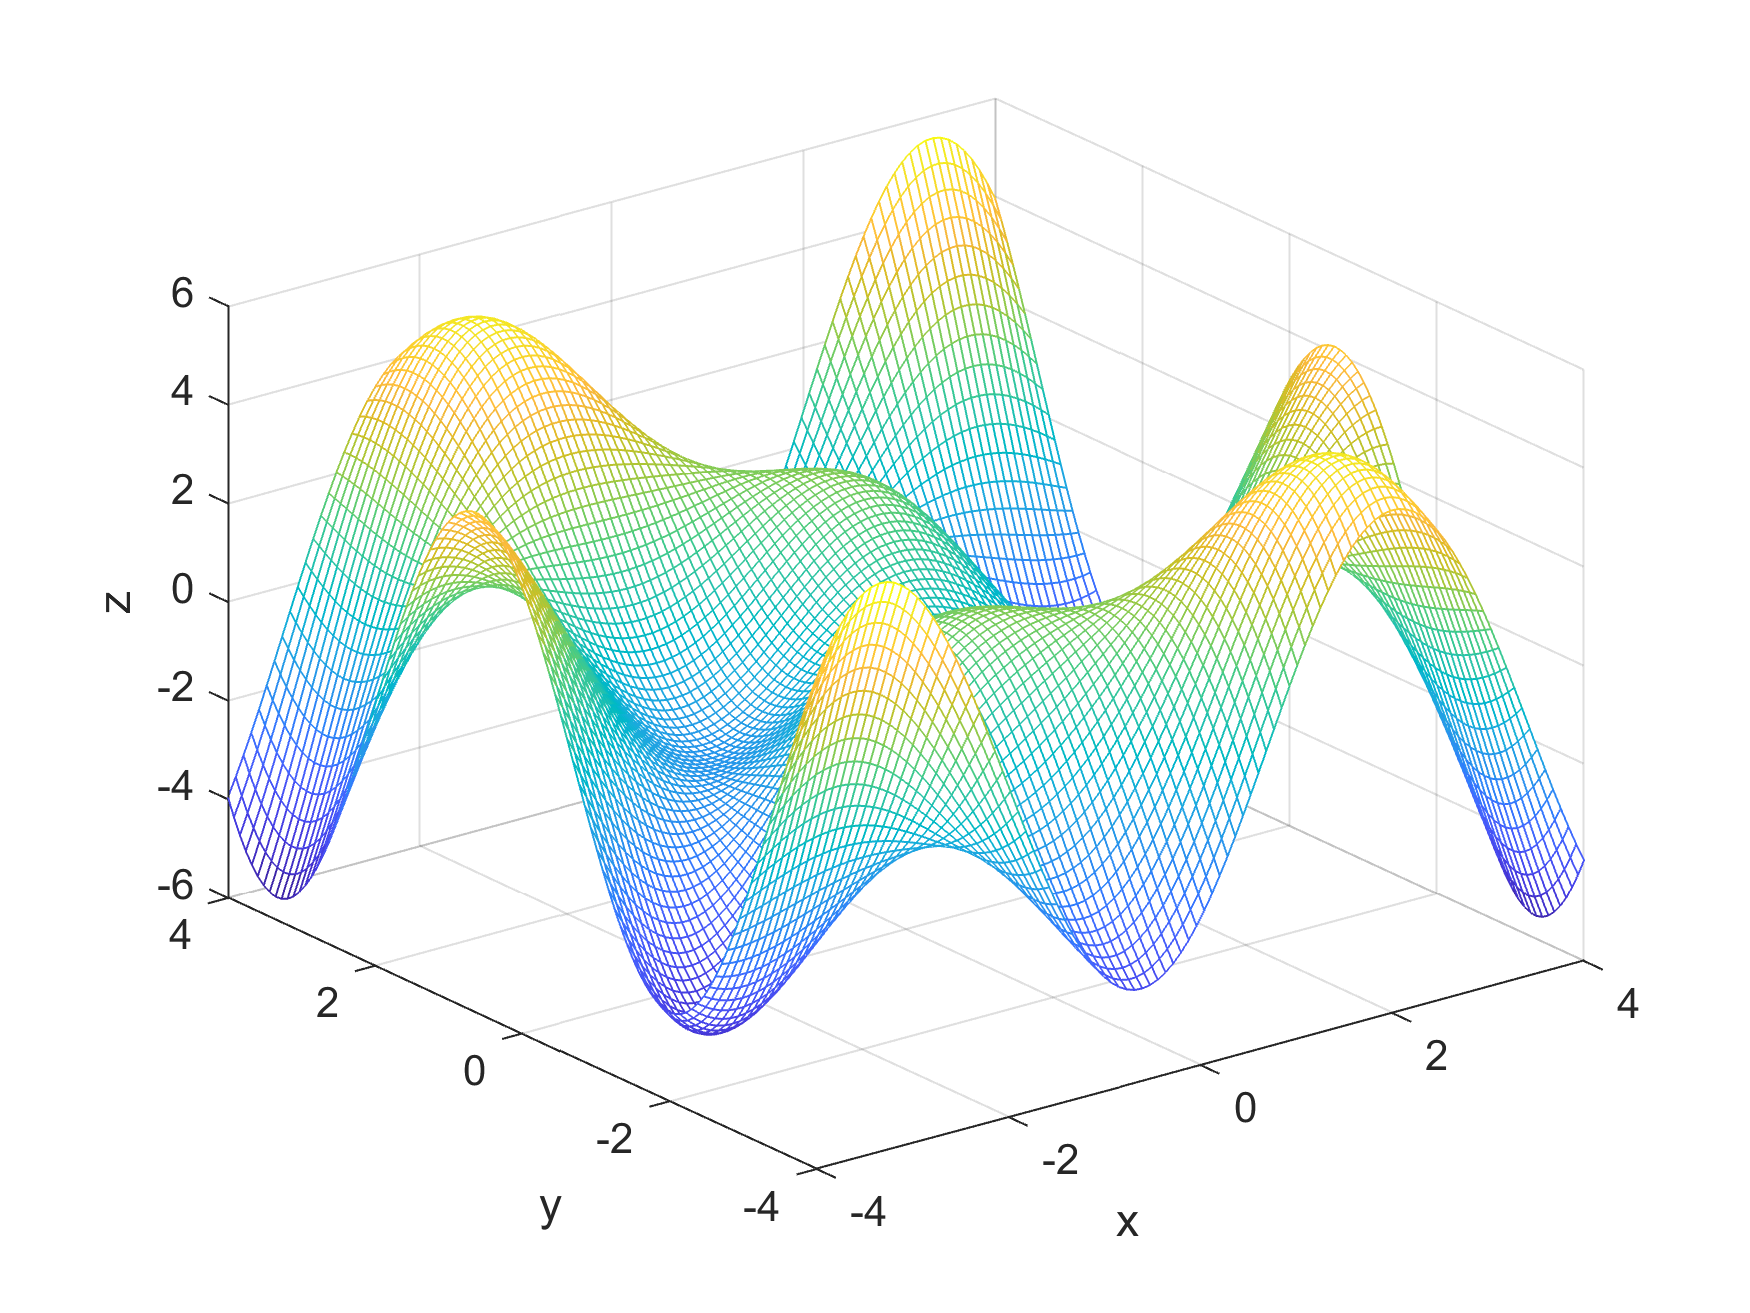
\includegraphics[width=12cm]{Q1/figures/3Dplot.png}
\end{figure}
\begin{figure}[H]
	\caption{3D figure of function with Points}
	\centering
	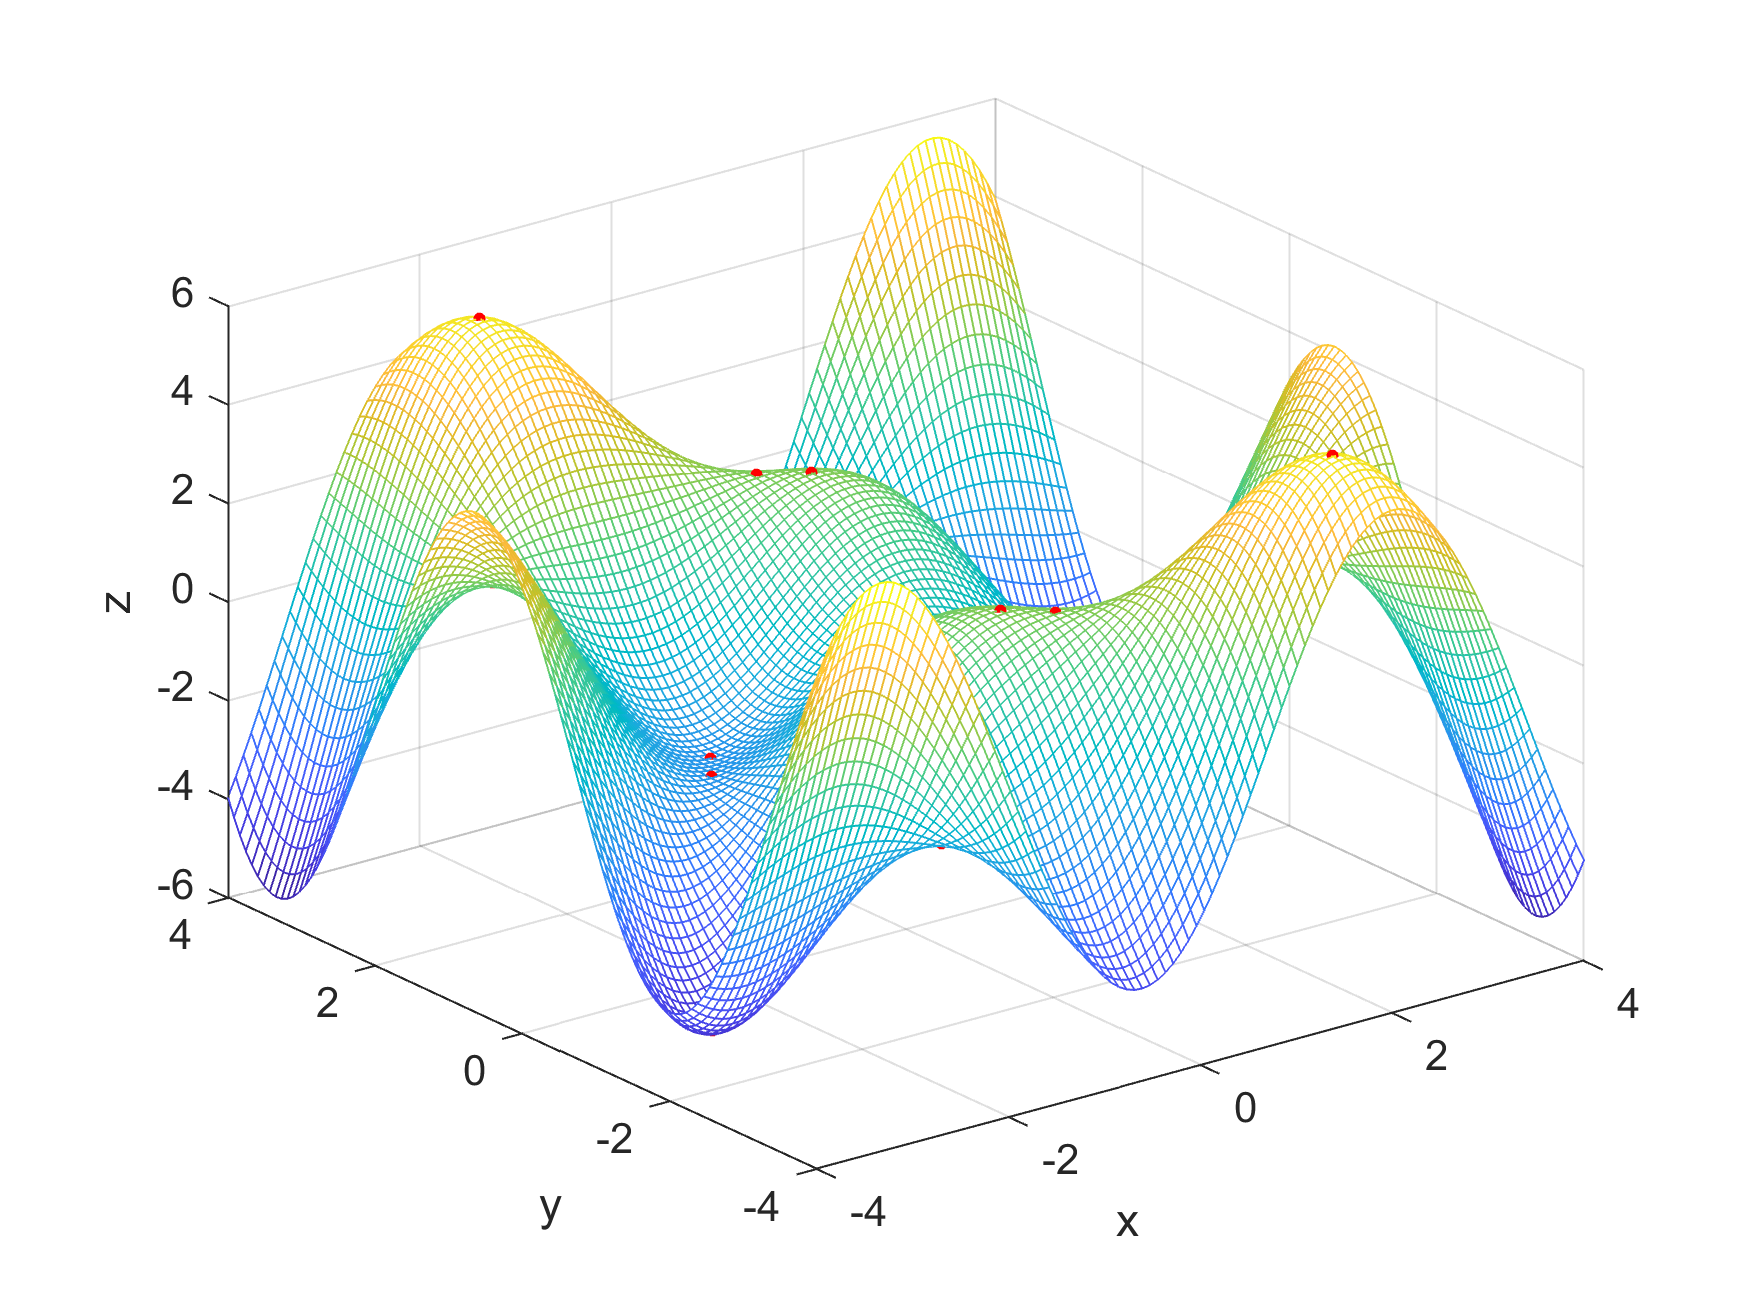
\includegraphics[width=12cm]{Q1/figures/3DplotWithPoints.png}
\end{figure}
\begin{figure}[H]
	\caption{Contour figure of function}
	\centering
	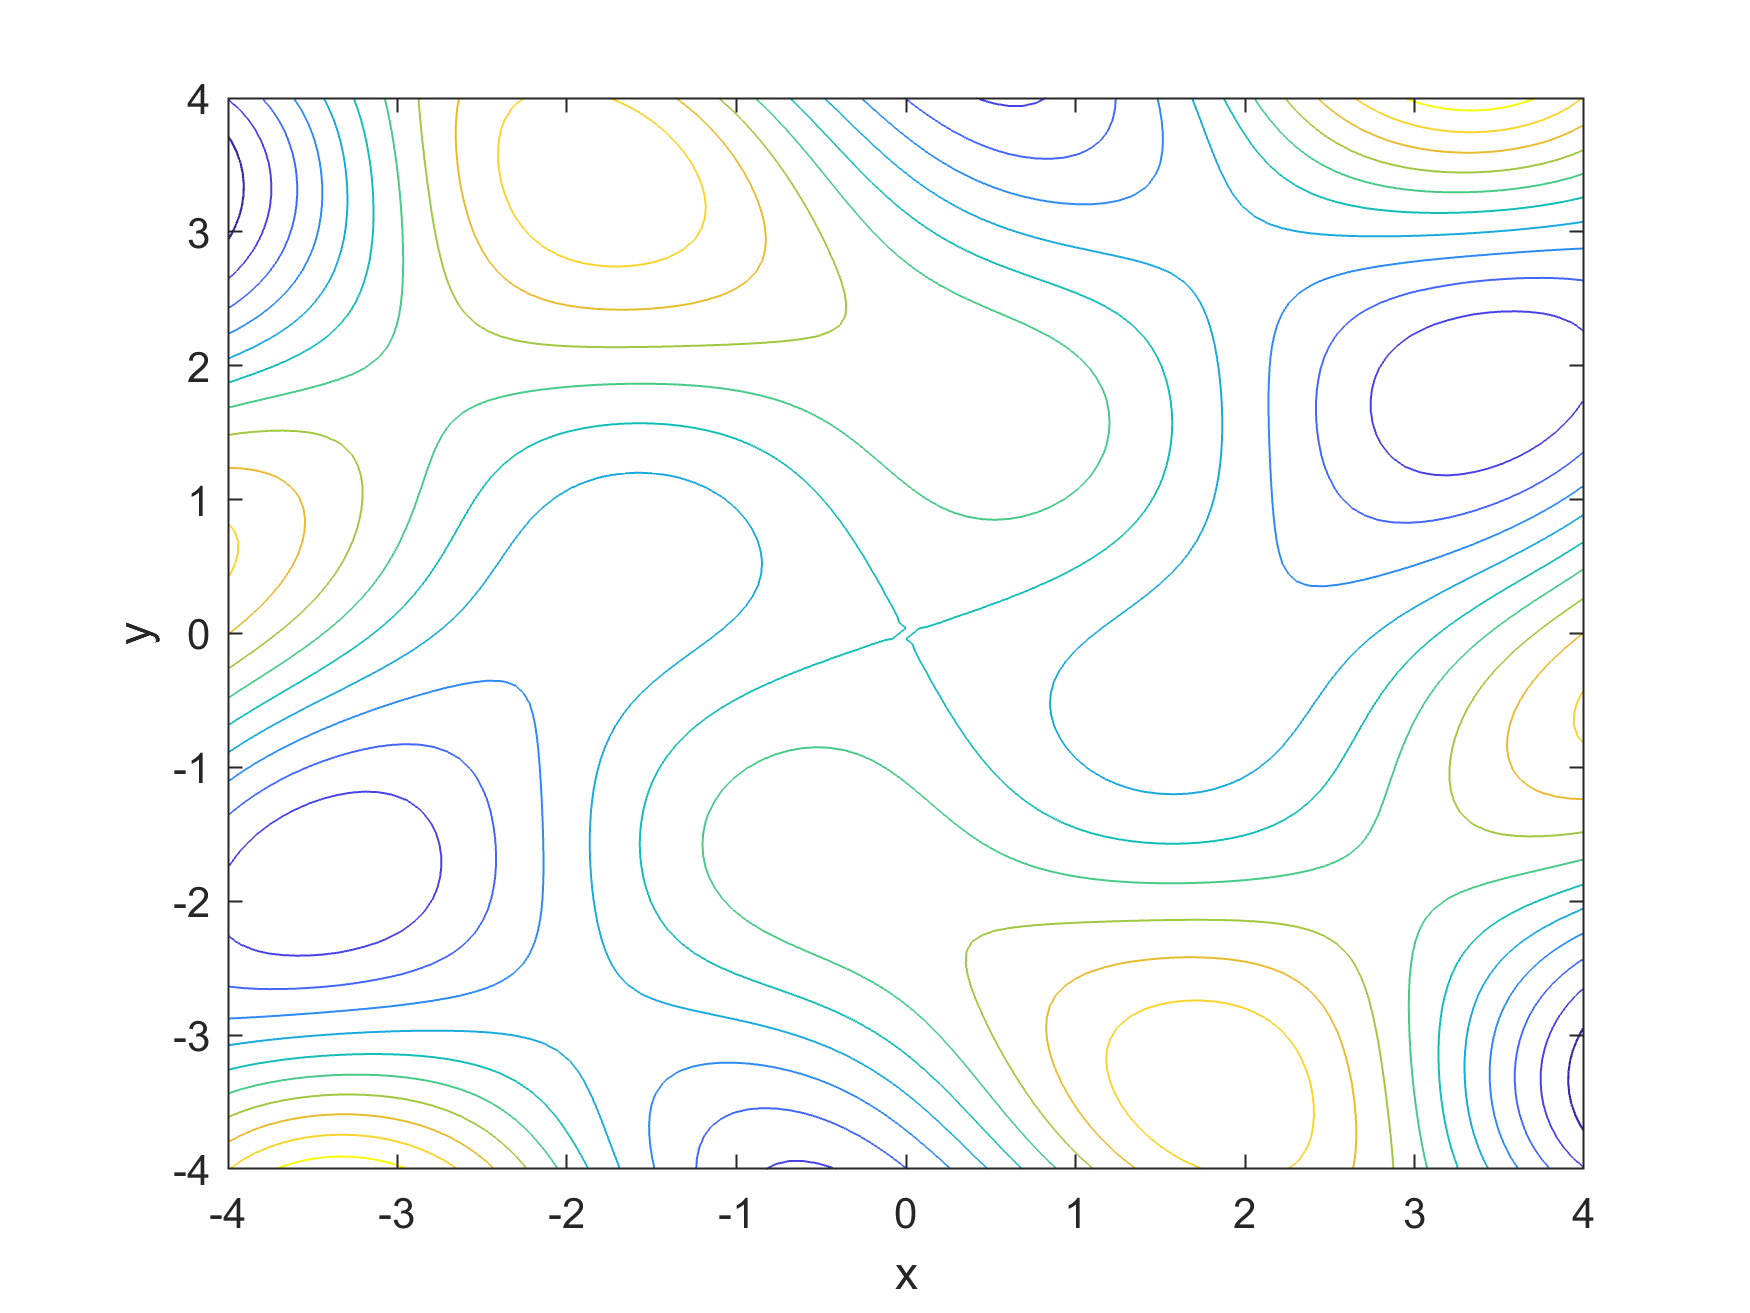
\includegraphics[width=12cm]{Q1/figures/Contour.png}
\end{figure}
\begin{figure}[H]
	\caption{Contour figure of function with Points}
	\centering
	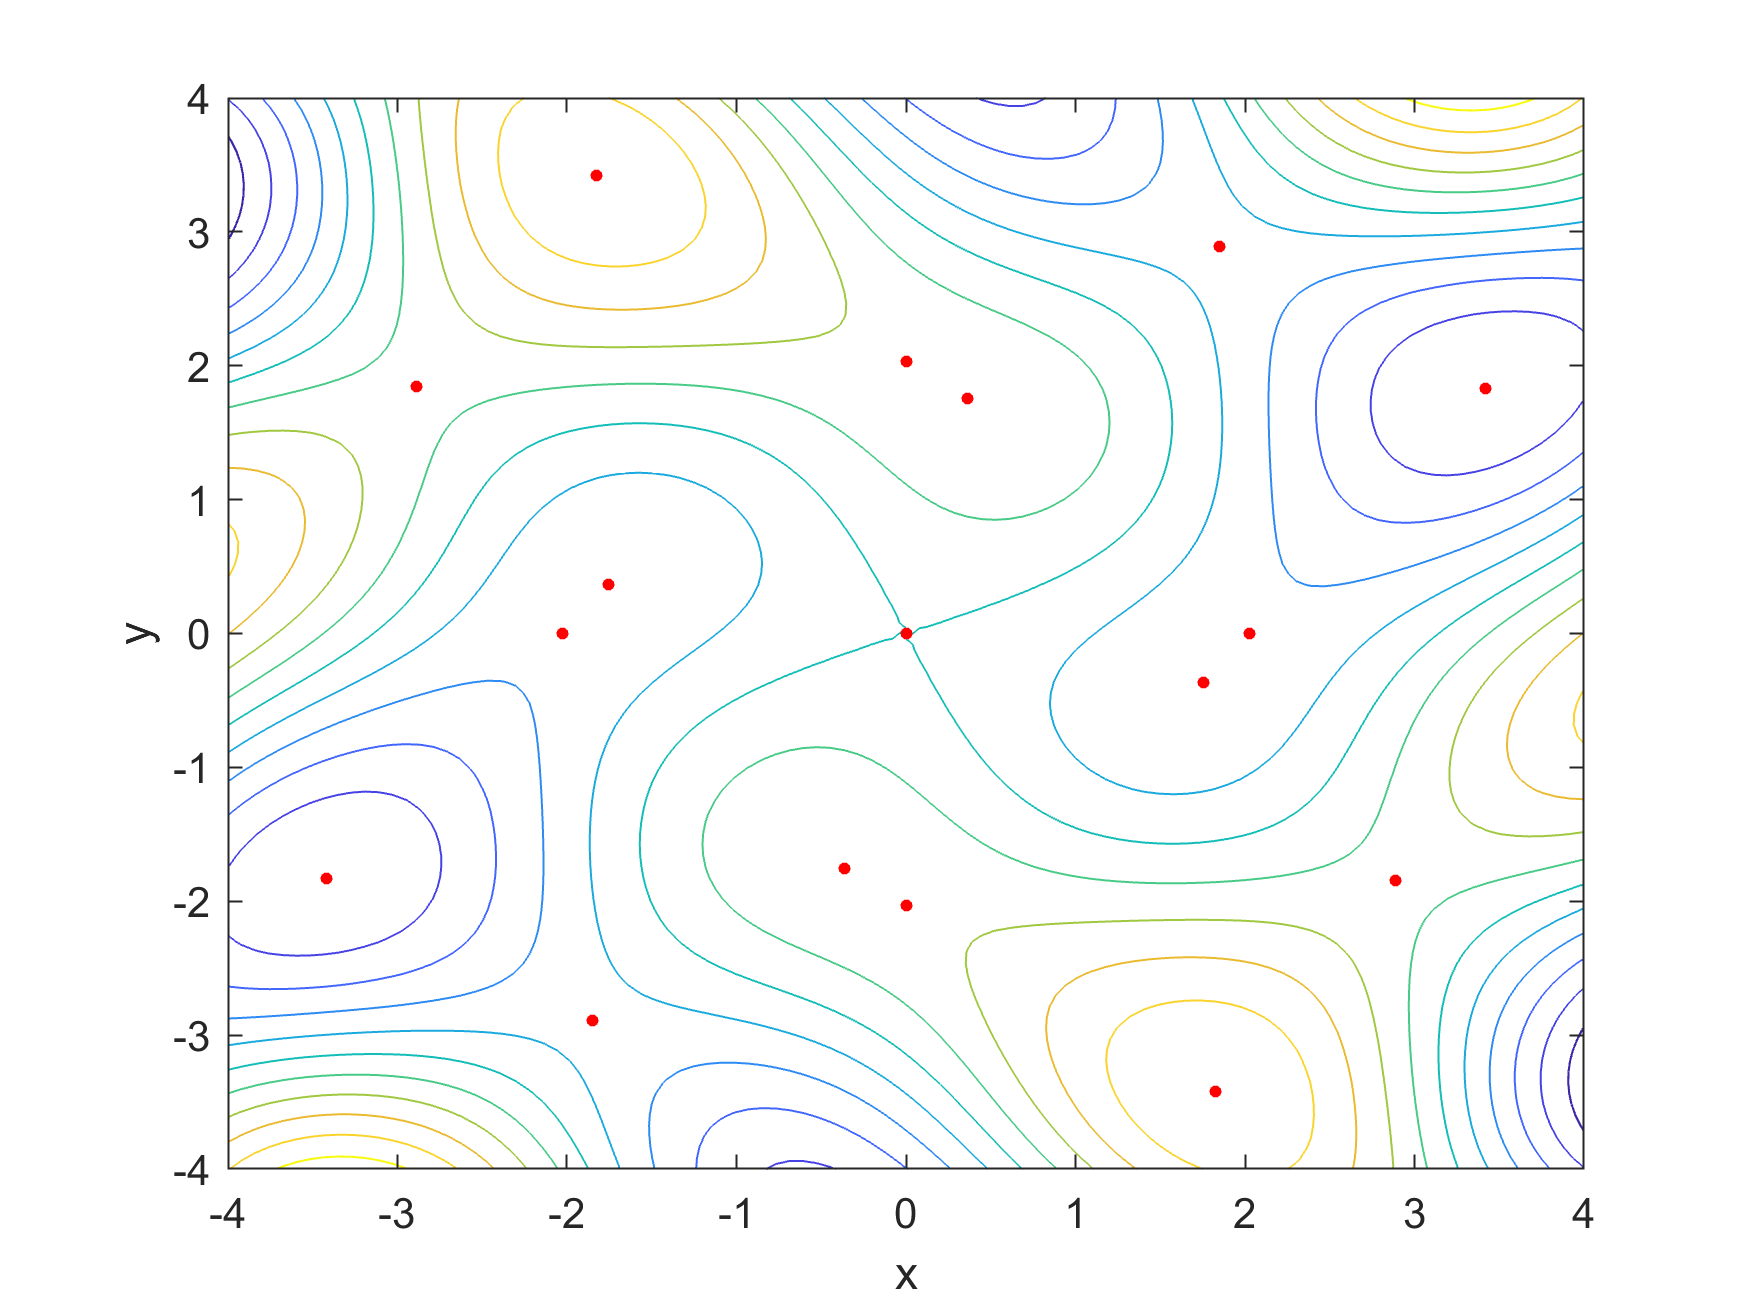
\includegraphics[width=12cm]{Q1/figures/ContourWithPoints.png}
\end{figure}

